\documentclass[]{article}
\usepackage{lmodern}
\usepackage{amssymb,amsmath}
\usepackage{ifxetex,ifluatex}
\usepackage{fixltx2e} % provides \textsubscript
\ifnum 0\ifxetex 1\fi\ifluatex 1\fi=0 % if pdftex
  \usepackage[T1]{fontenc}
  \usepackage[utf8]{inputenc}
\else % if luatex or xelatex
  \ifxetex
    \usepackage{mathspec}
  \else
    \usepackage{fontspec}
  \fi
  \defaultfontfeatures{Ligatures=TeX,Scale=MatchLowercase}
\fi
% use upquote if available, for straight quotes in verbatim environments
\IfFileExists{upquote.sty}{\usepackage{upquote}}{}
% use microtype if available
\IfFileExists{microtype.sty}{%
\usepackage{microtype}
\UseMicrotypeSet[protrusion]{basicmath} % disable protrusion for tt fonts
}{}
\usepackage[margin=1in]{geometry}
\usepackage{hyperref}
\hypersetup{unicode=true,
            pdfborder={0 0 0},
            breaklinks=true}
\urlstyle{same}  % don't use monospace font for urls
\usepackage{color}
\usepackage{fancyvrb}
\newcommand{\VerbBar}{|}
\newcommand{\VERB}{\Verb[commandchars=\\\{\}]}
\DefineVerbatimEnvironment{Highlighting}{Verbatim}{commandchars=\\\{\}}
% Add ',fontsize=\small' for more characters per line
\usepackage{framed}
\definecolor{shadecolor}{RGB}{248,248,248}
\newenvironment{Shaded}{\begin{snugshade}}{\end{snugshade}}
\newcommand{\AlertTok}[1]{\textcolor[rgb]{0.94,0.16,0.16}{#1}}
\newcommand{\AnnotationTok}[1]{\textcolor[rgb]{0.56,0.35,0.01}{\textbf{\textit{#1}}}}
\newcommand{\AttributeTok}[1]{\textcolor[rgb]{0.77,0.63,0.00}{#1}}
\newcommand{\BaseNTok}[1]{\textcolor[rgb]{0.00,0.00,0.81}{#1}}
\newcommand{\BuiltInTok}[1]{#1}
\newcommand{\CharTok}[1]{\textcolor[rgb]{0.31,0.60,0.02}{#1}}
\newcommand{\CommentTok}[1]{\textcolor[rgb]{0.56,0.35,0.01}{\textit{#1}}}
\newcommand{\CommentVarTok}[1]{\textcolor[rgb]{0.56,0.35,0.01}{\textbf{\textit{#1}}}}
\newcommand{\ConstantTok}[1]{\textcolor[rgb]{0.00,0.00,0.00}{#1}}
\newcommand{\ControlFlowTok}[1]{\textcolor[rgb]{0.13,0.29,0.53}{\textbf{#1}}}
\newcommand{\DataTypeTok}[1]{\textcolor[rgb]{0.13,0.29,0.53}{#1}}
\newcommand{\DecValTok}[1]{\textcolor[rgb]{0.00,0.00,0.81}{#1}}
\newcommand{\DocumentationTok}[1]{\textcolor[rgb]{0.56,0.35,0.01}{\textbf{\textit{#1}}}}
\newcommand{\ErrorTok}[1]{\textcolor[rgb]{0.64,0.00,0.00}{\textbf{#1}}}
\newcommand{\ExtensionTok}[1]{#1}
\newcommand{\FloatTok}[1]{\textcolor[rgb]{0.00,0.00,0.81}{#1}}
\newcommand{\FunctionTok}[1]{\textcolor[rgb]{0.00,0.00,0.00}{#1}}
\newcommand{\ImportTok}[1]{#1}
\newcommand{\InformationTok}[1]{\textcolor[rgb]{0.56,0.35,0.01}{\textbf{\textit{#1}}}}
\newcommand{\KeywordTok}[1]{\textcolor[rgb]{0.13,0.29,0.53}{\textbf{#1}}}
\newcommand{\NormalTok}[1]{#1}
\newcommand{\OperatorTok}[1]{\textcolor[rgb]{0.81,0.36,0.00}{\textbf{#1}}}
\newcommand{\OtherTok}[1]{\textcolor[rgb]{0.56,0.35,0.01}{#1}}
\newcommand{\PreprocessorTok}[1]{\textcolor[rgb]{0.56,0.35,0.01}{\textit{#1}}}
\newcommand{\RegionMarkerTok}[1]{#1}
\newcommand{\SpecialCharTok}[1]{\textcolor[rgb]{0.00,0.00,0.00}{#1}}
\newcommand{\SpecialStringTok}[1]{\textcolor[rgb]{0.31,0.60,0.02}{#1}}
\newcommand{\StringTok}[1]{\textcolor[rgb]{0.31,0.60,0.02}{#1}}
\newcommand{\VariableTok}[1]{\textcolor[rgb]{0.00,0.00,0.00}{#1}}
\newcommand{\VerbatimStringTok}[1]{\textcolor[rgb]{0.31,0.60,0.02}{#1}}
\newcommand{\WarningTok}[1]{\textcolor[rgb]{0.56,0.35,0.01}{\textbf{\textit{#1}}}}
\usepackage{graphicx,grffile}
\makeatletter
\def\maxwidth{\ifdim\Gin@nat@width>\linewidth\linewidth\else\Gin@nat@width\fi}
\def\maxheight{\ifdim\Gin@nat@height>\textheight\textheight\else\Gin@nat@height\fi}
\makeatother
% Scale images if necessary, so that they will not overflow the page
% margins by default, and it is still possible to overwrite the defaults
% using explicit options in \includegraphics[width, height, ...]{}
\setkeys{Gin}{width=\maxwidth,height=\maxheight,keepaspectratio}
\IfFileExists{parskip.sty}{%
\usepackage{parskip}
}{% else
\setlength{\parindent}{0pt}
\setlength{\parskip}{6pt plus 2pt minus 1pt}
}
\setlength{\emergencystretch}{3em}  % prevent overfull lines
\providecommand{\tightlist}{%
  \setlength{\itemsep}{0pt}\setlength{\parskip}{0pt}}
\setcounter{secnumdepth}{0}
% Redefines (sub)paragraphs to behave more like sections
\ifx\paragraph\undefined\else
\let\oldparagraph\paragraph
\renewcommand{\paragraph}[1]{\oldparagraph{#1}\mbox{}}
\fi
\ifx\subparagraph\undefined\else
\let\oldsubparagraph\subparagraph
\renewcommand{\subparagraph}[1]{\oldsubparagraph{#1}\mbox{}}
\fi

%%% Use protect on footnotes to avoid problems with footnotes in titles
\let\rmarkdownfootnote\footnote%
\def\footnote{\protect\rmarkdownfootnote}

%%% Change title format to be more compact
\usepackage{titling}

% Create subtitle command for use in maketitle
\providecommand{\subtitle}[1]{
  \posttitle{
    \begin{center}\large#1\end{center}
    }
}

\setlength{\droptitle}{-2em}

  \title{}
    \pretitle{\vspace{\droptitle}}
  \posttitle{}
    \author{}
    \preauthor{}\postauthor{}
    \date{}
    \predate{}\postdate{}
  

\begin{document}

Uploading the libraries

\begin{Shaded}
\begin{Highlighting}[]
\KeywordTok{library}\NormalTok{(mosaic)}
\end{Highlighting}
\end{Shaded}

\begin{verbatim}
## Loading required package: dplyr
\end{verbatim}

\begin{verbatim}
## 
## Attaching package: 'dplyr'
\end{verbatim}

\begin{verbatim}
## The following objects are masked from 'package:stats':
## 
##     filter, lag
\end{verbatim}

\begin{verbatim}
## The following objects are masked from 'package:base':
## 
##     intersect, setdiff, setequal, union
\end{verbatim}

\begin{verbatim}
## Loading required package: lattice
\end{verbatim}

\begin{verbatim}
## Loading required package: ggformula
\end{verbatim}

\begin{verbatim}
## Loading required package: ggplot2
\end{verbatim}

\begin{verbatim}
## Loading required package: ggstance
\end{verbatim}

\begin{verbatim}
## 
## Attaching package: 'ggstance'
\end{verbatim}

\begin{verbatim}
## The following objects are masked from 'package:ggplot2':
## 
##     geom_errorbarh, GeomErrorbarh
\end{verbatim}

\begin{verbatim}
## 
## New to ggformula?  Try the tutorials: 
##  learnr::run_tutorial("introduction", package = "ggformula")
##  learnr::run_tutorial("refining", package = "ggformula")
\end{verbatim}

\begin{verbatim}
## Loading required package: mosaicData
\end{verbatim}

\begin{verbatim}
## Loading required package: Matrix
\end{verbatim}

\begin{verbatim}
## Registered S3 method overwritten by 'mosaic':
##   method                           from   
##   fortify.SpatialPolygonsDataFrame ggplot2
\end{verbatim}

\begin{verbatim}
## 
## The 'mosaic' package masks several functions from core packages in order to add 
## additional features.  The original behavior of these functions should not be affected by this.
## 
## Note: If you use the Matrix package, be sure to load it BEFORE loading mosaic.
\end{verbatim}

\begin{verbatim}
## 
## Attaching package: 'mosaic'
\end{verbatim}

\begin{verbatim}
## The following object is masked from 'package:Matrix':
## 
##     mean
\end{verbatim}

\begin{verbatim}
## The following object is masked from 'package:ggplot2':
## 
##     stat
\end{verbatim}

\begin{verbatim}
## The following objects are masked from 'package:dplyr':
## 
##     count, do, tally
\end{verbatim}

\begin{verbatim}
## The following objects are masked from 'package:stats':
## 
##     binom.test, cor, cor.test, cov, fivenum, IQR, median,
##     prop.test, quantile, sd, t.test, var
\end{verbatim}

\begin{verbatim}
## The following objects are masked from 'package:base':
## 
##     max, mean, min, prod, range, sample, sum
\end{verbatim}

\begin{Shaded}
\begin{Highlighting}[]
\KeywordTok{library}\NormalTok{(quantmod)}
\end{Highlighting}
\end{Shaded}

\begin{verbatim}
## Loading required package: xts
\end{verbatim}

\begin{verbatim}
## Loading required package: zoo
\end{verbatim}

\begin{verbatim}
## 
## Attaching package: 'zoo'
\end{verbatim}

\begin{verbatim}
## The following objects are masked from 'package:base':
## 
##     as.Date, as.Date.numeric
\end{verbatim}

\begin{verbatim}
## Registered S3 method overwritten by 'xts':
##   method     from
##   as.zoo.xts zoo
\end{verbatim}

\begin{verbatim}
## 
## Attaching package: 'xts'
\end{verbatim}

\begin{verbatim}
## The following objects are masked from 'package:dplyr':
## 
##     first, last
\end{verbatim}

\begin{verbatim}
## Loading required package: TTR
\end{verbatim}

\begin{verbatim}
## Registered S3 method overwritten by 'quantmod':
##   method            from
##   as.zoo.data.frame zoo
\end{verbatim}

\begin{verbatim}
## Version 0.4-0 included new data defaults. See ?getSymbols.
\end{verbatim}

\begin{Shaded}
\begin{Highlighting}[]
\KeywordTok{library}\NormalTok{(foreach)}
\end{Highlighting}
\end{Shaded}

Importing the stocks that we want to use

\begin{Shaded}
\begin{Highlighting}[]
\NormalTok{port1 <-}\StringTok{ }\KeywordTok{c}\NormalTok{(}\StringTok{"EDEN"}\NormalTok{, }\StringTok{"GXC"}\NormalTok{, }\StringTok{"CXSE"}\NormalTok{, }\StringTok{"QEMM"}\NormalTok{, }\StringTok{"IEMG"}\NormalTok{)}

\NormalTok{port2 <-}\StringTok{ }\KeywordTok{c}\NormalTok{(}\StringTok{"FSZ"}\NormalTok{, }\StringTok{"JPMV"}\NormalTok{,  }\StringTok{"FCA"}\NormalTok{, }\StringTok{"TUR"}\NormalTok{)}

\NormalTok{port3 <-}\StringTok{ }\KeywordTok{c}\NormalTok{(}\StringTok{"EWJ"}\NormalTok{, }\StringTok{"EWL"}\NormalTok{, }\StringTok{"EWN"}\NormalTok{, }\StringTok{"ASHR"}\NormalTok{, }\StringTok{"KFYP"}\NormalTok{, }\StringTok{"GREK"}\NormalTok{, }\StringTok{"ERUS"}\NormalTok{)}

\NormalTok{port1.data <-}\StringTok{ }\KeywordTok{getSymbols}\NormalTok{(port1, }\DataTypeTok{from =} \StringTok{"2014-01-01"}\NormalTok{)}
\end{Highlighting}
\end{Shaded}

\begin{verbatim}
## 'getSymbols' currently uses auto.assign=TRUE by default, but will
## use auto.assign=FALSE in 0.5-0. You will still be able to use
## 'loadSymbols' to automatically load data. getOption("getSymbols.env")
## and getOption("getSymbols.auto.assign") will still be checked for
## alternate defaults.
## 
## This message is shown once per session and may be disabled by setting 
## options("getSymbols.warning4.0"=FALSE). See ?getSymbols for details.
\end{verbatim}

\begin{Shaded}
\begin{Highlighting}[]
\NormalTok{port2.data <-}\StringTok{ }\KeywordTok{getSymbols}\NormalTok{(port2, }\DataTypeTok{from =} \StringTok{"2014-01-01"}\NormalTok{)}
\NormalTok{port3.data <-}\StringTok{ }\KeywordTok{getSymbols}\NormalTok{(port3, }\DataTypeTok{from =} \StringTok{"2014-01-01"}\NormalTok{)}
\end{Highlighting}
\end{Shaded}

\begin{verbatim}
## pausing 1 second between requests for more than 5 symbols
\end{verbatim}

\begin{verbatim}
## pausing 1 second between requests for more than 5 symbols
## pausing 1 second between requests for more than 5 symbols
\end{verbatim}

Adjusting for splits and dividends

\begin{Shaded}
\begin{Highlighting}[]
\NormalTok{EDENa <-}\StringTok{ }\KeywordTok{adjustOHLC}\NormalTok{(EDEN)}
\NormalTok{GXCa <-}\StringTok{ }\KeywordTok{adjustOHLC}\NormalTok{(GXC)}
\NormalTok{CXSEa <-}\StringTok{ }\KeywordTok{adjustOHLC}\NormalTok{(CXSE)}
\NormalTok{QEMMa <-}\StringTok{ }\KeywordTok{adjustOHLC}\NormalTok{(QEMM)}
\NormalTok{IEMGa <-}\StringTok{ }\KeywordTok{adjustOHLC}\NormalTok{(IEMG)}

\NormalTok{FSZb <-}\StringTok{ }\KeywordTok{adjustOHLC}\NormalTok{(FSZ)}
\NormalTok{JPMVb <-}\StringTok{ }\KeywordTok{adjustOHLC}\NormalTok{(JPMV)}
\NormalTok{FCAb <-}\StringTok{ }\KeywordTok{adjustOHLC}\NormalTok{(FCA)}
\NormalTok{TURb <-}\StringTok{ }\KeywordTok{adjustOHLC}\NormalTok{(TUR)}

\NormalTok{EWJc <-}\StringTok{ }\KeywordTok{adjustOHLC}\NormalTok{(EWJ)}
\NormalTok{EWLc <-}\StringTok{ }\KeywordTok{adjustOHLC}\NormalTok{(EWL)}
\NormalTok{EWNc <-}\StringTok{ }\KeywordTok{adjustOHLC}\NormalTok{(EWN)}
\NormalTok{ASHRc <-}\StringTok{ }\KeywordTok{adjustOHLC}\NormalTok{(ASHR)}
\NormalTok{KFYPc <-}\StringTok{ }\KeywordTok{adjustOHLC}\NormalTok{(KFYP)}
\NormalTok{GREKc <-}\StringTok{ }\KeywordTok{adjustOHLC}\NormalTok{(GREK)}
\NormalTok{ERUSc <-}\StringTok{ }\KeywordTok{adjustOHLC}\NormalTok{(ERUS)}
\end{Highlighting}
\end{Shaded}

Combining close to close changes in a single matrix

\begin{Shaded}
\begin{Highlighting}[]
\NormalTok{all_returns_a <-}\StringTok{ }\KeywordTok{cbind}\NormalTok{(}\KeywordTok{ClCl}\NormalTok{(EDENa),}\KeywordTok{ClCl}\NormalTok{(GXCa), }\KeywordTok{ClCl}\NormalTok{(CXSEa),}\KeywordTok{ClCl}\NormalTok{(QEMMa),}\KeywordTok{ClCl}\NormalTok{(IEMGa))}
\NormalTok{all_returns_b <-}\StringTok{ }\KeywordTok{cbind}\NormalTok{(}\KeywordTok{ClCl}\NormalTok{(FSZb),}\KeywordTok{ClCl}\NormalTok{(JPMVb), }\KeywordTok{ClCl}\NormalTok{(FCAb),}\KeywordTok{ClCl}\NormalTok{(TURb))}
\NormalTok{all_returns_c <-}\StringTok{ }\KeywordTok{cbind}\NormalTok{(}\KeywordTok{ClCl}\NormalTok{(EWJc),}\KeywordTok{ClCl}\NormalTok{(EWLc), }\KeywordTok{ClCl}\NormalTok{(EWNc),}\KeywordTok{ClCl}\NormalTok{(ASHRc),}\KeywordTok{ClCl}\NormalTok{(KFYPc),}\KeywordTok{ClCl}\NormalTok{(GREKc),}\KeywordTok{ClCl}\NormalTok{(ERUSc))}

\NormalTok{all_returns_a =}\StringTok{ }\KeywordTok{as.matrix}\NormalTok{(}\KeywordTok{na.omit}\NormalTok{(all_returns_a))}
\NormalTok{all_returns_b =}\StringTok{ }\KeywordTok{as.matrix}\NormalTok{(}\KeywordTok{na.omit}\NormalTok{(all_returns_b))}
\NormalTok{all_returns_c =}\StringTok{ }\KeywordTok{as.matrix}\NormalTok{(}\KeywordTok{na.omit}\NormalTok{(all_returns_c))}

\KeywordTok{print}\NormalTok{(}\StringTok{"Portfolio a: "}\NormalTok{)}
\end{Highlighting}
\end{Shaded}

\begin{verbatim}
## [1] "Portfolio a: "
\end{verbatim}

\begin{Shaded}
\begin{Highlighting}[]
\KeywordTok{head}\NormalTok{(all_returns_a)}
\end{Highlighting}
\end{Shaded}

\begin{verbatim}
##               ClCl.EDENa     ClCl.GXCa    ClCl.CXSEa   ClCl.QEMMa
## 2014-06-06 -0.0022484355  0.0002689567 -0.0005862615  0.009933741
## 2014-06-09  0.0015023850  0.0084677014  0.0031286665 -0.002131164
## 2014-06-10  0.0007499906  0.0058643477  0.0077973101  0.000000000
## 2014-06-11 -0.0106801576 -0.0051676030 -0.0069632687  0.000000000
## 2014-06-12  0.0077651517 -0.0006659963 -0.0001947409  0.000000000
## 2014-06-13 -0.0052621501  0.0106624418  0.0126631205  0.018728422
##               ClCl.IEMGa
## 2014-06-06  0.0098951880
## 2014-06-09  0.0032661288
## 2014-06-10  0.0045959019
## 2014-06-11 -0.0032405262
## 2014-06-12 -0.0036336392
## 2014-06-13  0.0001919962
\end{verbatim}

\begin{Shaded}
\begin{Highlighting}[]
\KeywordTok{print}\NormalTok{(}\StringTok{""}\NormalTok{)}
\end{Highlighting}
\end{Shaded}

\begin{verbatim}
## [1] ""
\end{verbatim}

\begin{Shaded}
\begin{Highlighting}[]
\KeywordTok{print}\NormalTok{(}\StringTok{"Portfolio b: "}\NormalTok{)}
\end{Highlighting}
\end{Shaded}

\begin{verbatim}
## [1] "Portfolio b: "
\end{verbatim}

\begin{Shaded}
\begin{Highlighting}[]
\KeywordTok{head}\NormalTok{(all_returns_b)}
\end{Highlighting}
\end{Shaded}

\begin{verbatim}
##                ClCl.FSZb   ClCl.JPMVb     ClCl.FCAb    ClCl.TURb
## 2014-06-06 -0.0004515918  0.004694875 -0.0045641716  0.011635866
## 2014-06-09  0.0038400497 -0.007009365  0.0000000000  0.001860639
## 2014-06-10 -0.0045003826 -0.005098000  0.0050436041  0.013000169
## 2014-06-11 -0.0099458178  0.002759145 -0.0018248631 -0.051999983
## 2014-06-12  0.0002283562  0.007665075  0.0009141225  0.004043600
## 2014-06-13 -0.0034238986 -0.001755413  0.0000000000 -0.006303642
\end{verbatim}

\begin{Shaded}
\begin{Highlighting}[]
\KeywordTok{print}\NormalTok{(}\StringTok{""}\NormalTok{)}
\end{Highlighting}
\end{Shaded}

\begin{verbatim}
## [1] ""
\end{verbatim}

\begin{Shaded}
\begin{Highlighting}[]
\KeywordTok{print}\NormalTok{(}\StringTok{"Portfolio c: "}\NormalTok{)}
\end{Highlighting}
\end{Shaded}

\begin{verbatim}
## [1] "Portfolio c: "
\end{verbatim}

\begin{Shaded}
\begin{Highlighting}[]
\KeywordTok{head}\NormalTok{(all_returns_c)}
\end{Highlighting}
\end{Shaded}

\begin{verbatim}
##               ClCl.EWJc     ClCl.EWLc     ClCl.EWNc    ClCl.ASHRc
## 2014-01-03  0.005862710  0.0099348032 -0.0015673981 -0.0045454957
## 2014-01-06 -0.003330558 -0.0003073778 -0.0007849686 -0.0249066002
## 2014-01-07  0.004177130  0.0009224785  0.0062844464  0.0021286079
## 2014-01-08  0.001663852 -0.0012289094  0.0003902420  0.0004247239
## 2014-01-09 -0.003322259  0.0055367890  0.0011705424 -0.0148619115
## 2014-01-10  0.006666667  0.0104007345  0.0074045207  0.0073275859
##              ClCl.KFYPc   ClCl.GREKc   ClCl.ERUSc
## 2014-01-03 -0.010716442 -0.010118786 -0.005673712
## 2014-01-06 -0.001547601  0.004888933 -0.019495934
## 2014-01-07  0.002014972  0.026536841  0.004364597
## 2014-01-08  0.014385150  0.026712668 -0.002897127
## 2014-01-09  0.000000000  0.005874906 -0.005326804
## 2014-01-10  0.000000000  0.014184398  0.018500437
\end{verbatim}

Computing the returns from the closing prices

\begin{Shaded}
\begin{Highlighting}[]
\KeywordTok{pairs}\NormalTok{(all_returns_a)}
\end{Highlighting}
\end{Shaded}

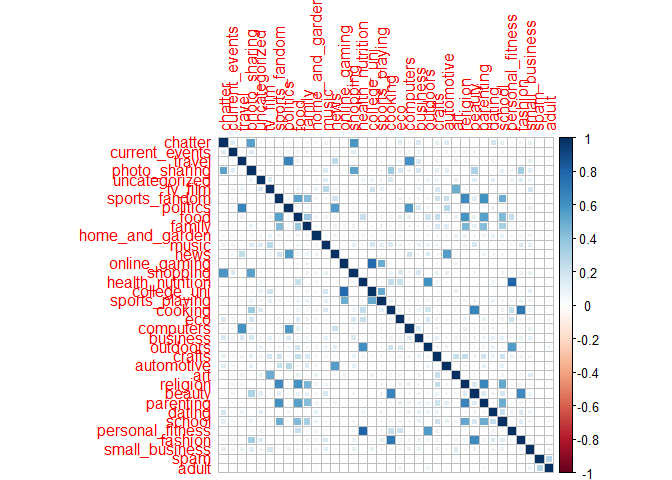
\includegraphics{finalproj_files/figure-latex/unnamed-chunk-5-1.pdf}

\begin{Shaded}
\begin{Highlighting}[]
\KeywordTok{pairs}\NormalTok{(all_returns_b)}
\end{Highlighting}
\end{Shaded}

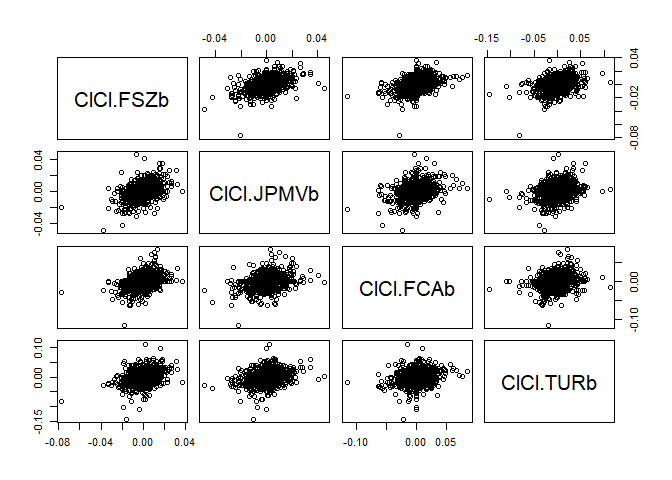
\includegraphics{finalproj_files/figure-latex/unnamed-chunk-5-2.pdf}

\begin{Shaded}
\begin{Highlighting}[]
\KeywordTok{pairs}\NormalTok{(all_returns_c)}
\end{Highlighting}
\end{Shaded}

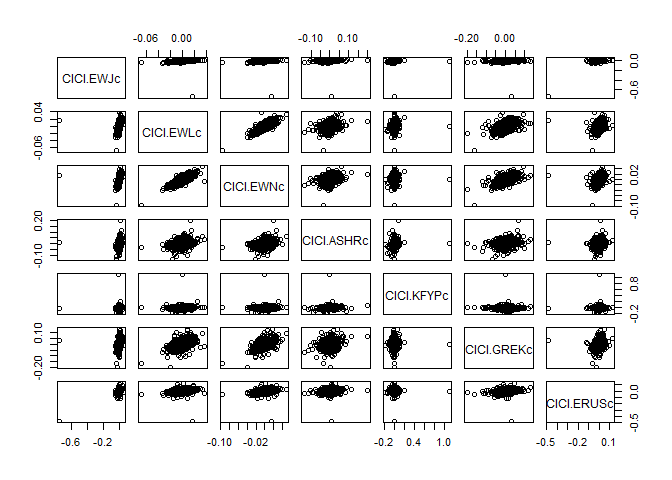
\includegraphics{finalproj_files/figure-latex/unnamed-chunk-5-3.pdf}
Sampling a random return from the empirical joint distribution

\begin{Shaded}
\begin{Highlighting}[]
\KeywordTok{set.seed}\NormalTok{(}\DecValTok{45}\NormalTok{)}
\NormalTok{return.today_a <-}\StringTok{ }\KeywordTok{resample}\NormalTok{(all_returns_a, }\DecValTok{1}\NormalTok{, }\DataTypeTok{orig.ids =} \OtherTok{FALSE}\NormalTok{)}
\NormalTok{return.today_b <-}\StringTok{ }\KeywordTok{resample}\NormalTok{(all_returns_b, }\DecValTok{1}\NormalTok{, }\DataTypeTok{orig.ids =} \OtherTok{FALSE}\NormalTok{)}
\NormalTok{return.today_c <-}\StringTok{ }\KeywordTok{resample}\NormalTok{(all_returns_c, }\DecValTok{1}\NormalTok{, }\DataTypeTok{orig.ids =} \OtherTok{FALSE}\NormalTok{)}
\end{Highlighting}
\end{Shaded}

Update the value of my holdings, starting with an equal distribution to
each asset

\begin{Shaded}
\begin{Highlighting}[]
\KeywordTok{set.seed}\NormalTok{(}\DecValTok{45}\NormalTok{)}
\NormalTok{total_wealth =}\StringTok{ }\DecValTok{100000}
\NormalTok{my_weights_a <-}\StringTok{ }\KeywordTok{c}\NormalTok{(}\FloatTok{0.2}\NormalTok{, }\FloatTok{0.2}\NormalTok{, }\FloatTok{0.2}\NormalTok{, }\FloatTok{0.2}\NormalTok{, }\FloatTok{0.2}\NormalTok{)}
\NormalTok{my_weights_b <-}\StringTok{ }\KeywordTok{c}\NormalTok{(}\FloatTok{0.25}\NormalTok{, }\FloatTok{0.25}\NormalTok{, }\FloatTok{0.25}\NormalTok{, }\FloatTok{0.25}\NormalTok{)}
\NormalTok{my_weights_c <-}\StringTok{ }\KeywordTok{c}\NormalTok{(}\FloatTok{0.14}\NormalTok{, }\FloatTok{0.14}\NormalTok{, }\FloatTok{0.15}\NormalTok{, }\FloatTok{0.14}\NormalTok{, }\FloatTok{0.14}\NormalTok{, }\FloatTok{0.14}\NormalTok{, }\FloatTok{0.15}\NormalTok{)}

\NormalTok{holdings_a <-}\StringTok{ }\NormalTok{total_wealth}\OperatorTok{*}\NormalTok{my_weights_a}
\NormalTok{holdings_b <-}\StringTok{ }\NormalTok{total_wealth}\OperatorTok{*}\NormalTok{my_weights_b}
\NormalTok{holdings_c <-}\StringTok{ }\NormalTok{total_wealth}\OperatorTok{*}\NormalTok{my_weights_c}

\NormalTok{holdings_a <-}\StringTok{ }\NormalTok{holdings_a}\OperatorTok{*}\NormalTok{(}\DecValTok{1}\OperatorTok{+}\NormalTok{return.today_a)}
\NormalTok{holdings_b <-}\StringTok{ }\NormalTok{holdings_b}\OperatorTok{*}\NormalTok{(}\DecValTok{1}\OperatorTok{+}\NormalTok{return.today_b)}
\NormalTok{holdings_c <-}\StringTok{ }\NormalTok{holdings_c}\OperatorTok{*}\NormalTok{(}\DecValTok{1}\OperatorTok{+}\NormalTok{return.today_c)}

\NormalTok{total_wealth_a <-}\StringTok{ }\KeywordTok{sum}\NormalTok{(holdings_a)}
\NormalTok{total_wealth_b <-}\StringTok{ }\KeywordTok{sum}\NormalTok{(holdings_b)}
\NormalTok{total_weatlh_c <-}\StringTok{ }\KeywordTok{sum}\NormalTok{(holdings_c)}

\NormalTok{total_wealth_a}
\end{Highlighting}
\end{Shaded}

\begin{verbatim}
## [1] 100952.9
\end{verbatim}

\begin{Shaded}
\begin{Highlighting}[]
\NormalTok{total_wealth_b}
\end{Highlighting}
\end{Shaded}

\begin{verbatim}
## [1] 98416.81
\end{verbatim}

\begin{Shaded}
\begin{Highlighting}[]
\NormalTok{total_weatlh_c}
\end{Highlighting}
\end{Shaded}

\begin{verbatim}
## [1] 100240.9
\end{verbatim}

Loop over 4 trading weeks

\begin{Shaded}
\begin{Highlighting}[]
\KeywordTok{set.seed}\NormalTok{(}\DecValTok{45}\NormalTok{)}
\NormalTok{total_wealth =}\StringTok{ }\DecValTok{100000}
\NormalTok{my_weights_a <-}\StringTok{ }\KeywordTok{c}\NormalTok{(}\FloatTok{0.2}\NormalTok{, }\FloatTok{0.2}\NormalTok{, }\FloatTok{0.2}\NormalTok{, }\FloatTok{0.2}\NormalTok{, }\FloatTok{0.2}\NormalTok{)}
\NormalTok{my_weights_b <-}\StringTok{ }\KeywordTok{c}\NormalTok{(}\FloatTok{0.25}\NormalTok{, }\FloatTok{0.25}\NormalTok{, }\FloatTok{0.25}\NormalTok{, }\FloatTok{0.25}\NormalTok{)}
\NormalTok{my_weights_c <-}\StringTok{ }\KeywordTok{c}\NormalTok{(}\FloatTok{0.14}\NormalTok{, }\FloatTok{0.14}\NormalTok{, }\FloatTok{0.15}\NormalTok{, }\FloatTok{0.14}\NormalTok{, }\FloatTok{0.14}\NormalTok{, }\FloatTok{0.14}\NormalTok{, }\FloatTok{0.15}\NormalTok{)}

\NormalTok{holdings_a <-}\StringTok{ }\NormalTok{total_wealth}\OperatorTok{*}\NormalTok{my_weights_a}
\NormalTok{holdings_b <-}\StringTok{ }\NormalTok{total_wealth}\OperatorTok{*}\NormalTok{my_weights_b}
\NormalTok{holdings_c <-}\StringTok{ }\NormalTok{total_wealth}\OperatorTok{*}\NormalTok{my_weights_c}

\NormalTok{n_days =}\StringTok{ }\DecValTok{20}
\NormalTok{wealthtracker_a =}\StringTok{ }\KeywordTok{rep}\NormalTok{(}\DecValTok{0}\NormalTok{, n_days)}
\NormalTok{wealthtracker_b =}\StringTok{ }\KeywordTok{rep}\NormalTok{(}\DecValTok{0}\NormalTok{, n_days)}
\NormalTok{wealthtracker_c =}\StringTok{ }\KeywordTok{rep}\NormalTok{(}\DecValTok{0}\NormalTok{, n_days)}
\ControlFlowTok{for}\NormalTok{(today }\ControlFlowTok{in} \DecValTok{1}\OperatorTok{:}\NormalTok{n_days)\{}
\NormalTok{  return.today_a <-}\StringTok{ }\KeywordTok{resample}\NormalTok{(all_returns_a, }\DecValTok{1}\NormalTok{, }\DataTypeTok{orig.ids =} \OtherTok{FALSE}\NormalTok{)}
\NormalTok{  return.today_b <-}\StringTok{ }\KeywordTok{resample}\NormalTok{(all_returns_b, }\DecValTok{1}\NormalTok{, }\DataTypeTok{orig.ids =} \OtherTok{FALSE}\NormalTok{)}
\NormalTok{  return.today_c <-}\StringTok{ }\KeywordTok{resample}\NormalTok{(all_returns_c, }\DecValTok{1}\NormalTok{, }\DataTypeTok{orig.ids =} \OtherTok{FALSE}\NormalTok{) }
  
\NormalTok{  holdings_a <-}\StringTok{ }\NormalTok{holdings_a}\OperatorTok{*}\NormalTok{(}\DecValTok{1}\OperatorTok{+}\NormalTok{return.today_a)}
\NormalTok{  holdings_b <-}\StringTok{ }\NormalTok{holdings_b}\OperatorTok{*}\NormalTok{(}\DecValTok{1}\OperatorTok{+}\NormalTok{return.today_b)}
\NormalTok{  holdings_c <-}\StringTok{ }\NormalTok{holdings_c}\OperatorTok{*}\NormalTok{(}\DecValTok{1}\OperatorTok{+}\NormalTok{return.today_c)}
  
\NormalTok{  total_wealth_a <-}\StringTok{ }\KeywordTok{sum}\NormalTok{(holdings_a)}
\NormalTok{  total_wealth_b <-}\StringTok{ }\KeywordTok{sum}\NormalTok{(holdings_b)}
\NormalTok{  total_wealth_c <-}\StringTok{ }\KeywordTok{sum}\NormalTok{(holdings_c)}
  
\NormalTok{  wealthtracker_a[today] =}\StringTok{ }\NormalTok{total_wealth_a}
\NormalTok{  wealthtracker_b[today] =}\StringTok{ }\NormalTok{total_wealth_b}
\NormalTok{  wealthtracker_c[today] =}\StringTok{ }\NormalTok{total_wealth_c}
  
\NormalTok{\}}

\NormalTok{total_wealth_a}
\end{Highlighting}
\end{Shaded}

\begin{verbatim}
## [1] 100104.7
\end{verbatim}

\begin{Shaded}
\begin{Highlighting}[]
\NormalTok{total_wealth_b}
\end{Highlighting}
\end{Shaded}

\begin{verbatim}
## [1] 102691
\end{verbatim}

\begin{Shaded}
\begin{Highlighting}[]
\NormalTok{total_wealth_c}
\end{Highlighting}
\end{Shaded}

\begin{verbatim}
## [1] 94916.98
\end{verbatim}

\begin{Shaded}
\begin{Highlighting}[]
\KeywordTok{plot}\NormalTok{(wealthtracker_a, }\DataTypeTok{type =} \StringTok{'l'}\NormalTok{)}
\end{Highlighting}
\end{Shaded}

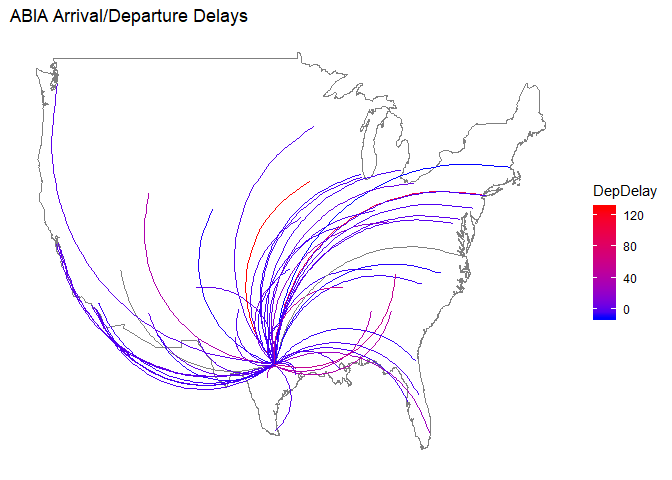
\includegraphics{finalproj_files/figure-latex/unnamed-chunk-8-1.pdf}

\begin{Shaded}
\begin{Highlighting}[]
\KeywordTok{plot}\NormalTok{(wealthtracker_b, }\DataTypeTok{type =} \StringTok{'l'}\NormalTok{)}
\end{Highlighting}
\end{Shaded}

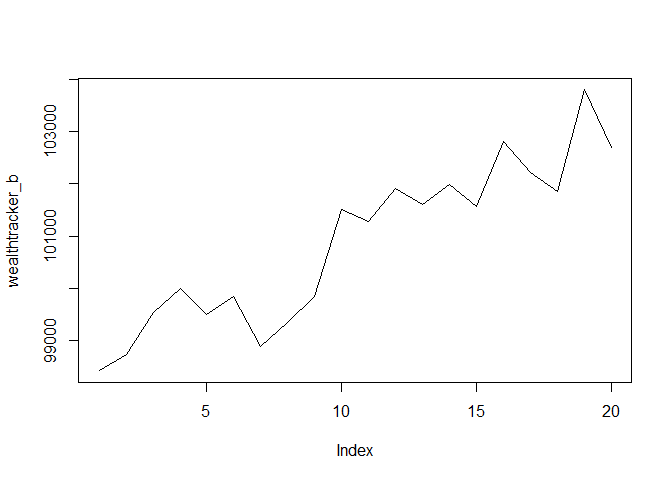
\includegraphics{finalproj_files/figure-latex/unnamed-chunk-8-2.pdf}

\begin{Shaded}
\begin{Highlighting}[]
\KeywordTok{plot}\NormalTok{(wealthtracker_c, }\DataTypeTok{type =} \StringTok{'l'}\NormalTok{)}
\end{Highlighting}
\end{Shaded}

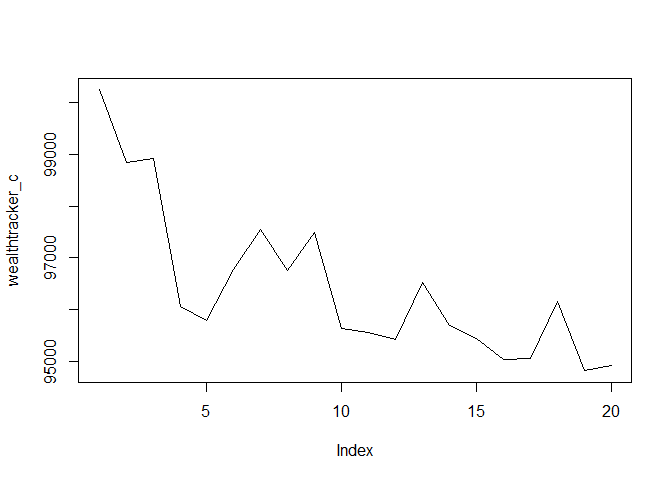
\includegraphics{finalproj_files/figure-latex/unnamed-chunk-8-3.pdf}

\begin{Shaded}
\begin{Highlighting}[]
\NormalTok{initial_wealth =}\StringTok{ }\DecValTok{100000}
\NormalTok{sim1 =}\StringTok{ }\KeywordTok{foreach}\NormalTok{(}\DataTypeTok{i =} \DecValTok{1}\OperatorTok{:}\DecValTok{5000}\NormalTok{, }\DataTypeTok{.combine =} \StringTok{"rbind"}\NormalTok{)}\OperatorTok\NormalTok{\{}
\NormalTok{  total_wealth_a =}\StringTok{ }\NormalTok{initial_wealth}
  
\NormalTok{  my_weights_a <-}\StringTok{ }\KeywordTok{c}\NormalTok{(}\FloatTok{0.2}\NormalTok{, }\FloatTok{0.2}\NormalTok{, }\FloatTok{0.2}\NormalTok{, }\FloatTok{0.2}\NormalTok{, }\FloatTok{0.2}\NormalTok{)}
  
\NormalTok{  holdings_a <-}\StringTok{ }\NormalTok{my_weights_a}\OperatorTok{*}\NormalTok{total_wealth_a}
  
\NormalTok{  n_days =}\StringTok{ }\DecValTok{20}
  
\NormalTok{  wealthtracker_a =}\StringTok{ }\KeywordTok{rep}\NormalTok{(}\DecValTok{0}\NormalTok{, n_days)}
  
  \ControlFlowTok{for}\NormalTok{(today }\ControlFlowTok{in} \DecValTok{1}\OperatorTok{:}\NormalTok{n_days)\{}
\NormalTok{    return.today_a <-}\StringTok{ }\KeywordTok{resample}\NormalTok{(all_returns_a, }\DecValTok{1}\NormalTok{, }\DataTypeTok{orig.ids =} \OtherTok{FALSE}\NormalTok{)}
  
\NormalTok{    holdings_a <-}\StringTok{ }\NormalTok{holdings_a}\OperatorTok{*}\NormalTok{(}\DecValTok{1}\OperatorTok{+}\NormalTok{return.today_a)}
  
\NormalTok{    total_wealth_a <-}\StringTok{ }\KeywordTok{sum}\NormalTok{(holdings_a)}
  
\NormalTok{    wealthtracker_a[today] =}\StringTok{ }\NormalTok{total_wealth_a}
\NormalTok{  \}}
\NormalTok{  wealthtracker_a}

  
\NormalTok{\}}
\KeywordTok{head}\NormalTok{(sim1)}
\end{Highlighting}
\end{Shaded}

\begin{verbatim}
##               [,1]      [,2]      [,3]      [,4]      [,5]      [,6]
## result.1  99611.53  99215.10  96809.80  95829.40  94317.40  95026.12
## result.2 100677.99 100197.70 100759.50 100213.31 100721.31 100073.47
## result.3  99555.35 101895.77 101604.30 100125.35 100437.51 100878.09
## result.4 100096.03  99941.09 100049.19  99433.99  99170.13  99957.07
## result.5  98752.10 100013.43  99277.66  99183.40 100457.08  99956.65
## result.6  99086.47  98486.74  98394.70  99334.17  99552.39  98368.74
##               [,7]      [,8]      [,9]     [,10]     [,11]     [,12]
## result.1  95191.21  95389.06  95061.64  95083.53  95234.81  95015.11
## result.2 100783.77 102213.67 102463.05 102584.80 103492.89 103461.98
## result.3 101579.25 101375.36 100967.65 101848.41 101182.62 102946.12
## result.4 101917.95 102457.05 100247.66 101473.53 100236.21 101972.58
## result.5  99375.63  99003.65 100114.64 100020.44 101238.63 100565.79
## result.6  98133.63  98892.87  98359.16  97850.92  97742.41  98408.11
##              [,13]     [,14]     [,15]     [,16]     [,17]     [,18]
## result.1  96168.49  96600.89  95607.15  93961.68  95424.29  95627.37
## result.2 103992.29 106263.77 104676.26 103821.54 104423.08 105469.43
## result.3 104679.86 105244.25 105026.39 107053.76 107224.22 106647.97
## result.4 102244.93 102151.25 102736.69 104108.61 103968.79 103530.06
## result.5 100883.92 101571.38 100841.96 100863.64 102028.27 102665.45
## result.6  99721.42  99748.20  99860.20 101479.76 101469.15 101007.98
##              [,19]    [,20]
## result.1  94948.52  93645.5
## result.2 105560.39 106219.1
## result.3 107018.03 105052.5
## result.4 101108.95 100888.2
## result.5 101728.17 101362.0
## result.6 101339.96  99795.8
\end{verbatim}

\begin{Shaded}
\begin{Highlighting}[]
\KeywordTok{hist}\NormalTok{(sim1[,n_days], }\DecValTok{25}\NormalTok{)}
\end{Highlighting}
\end{Shaded}

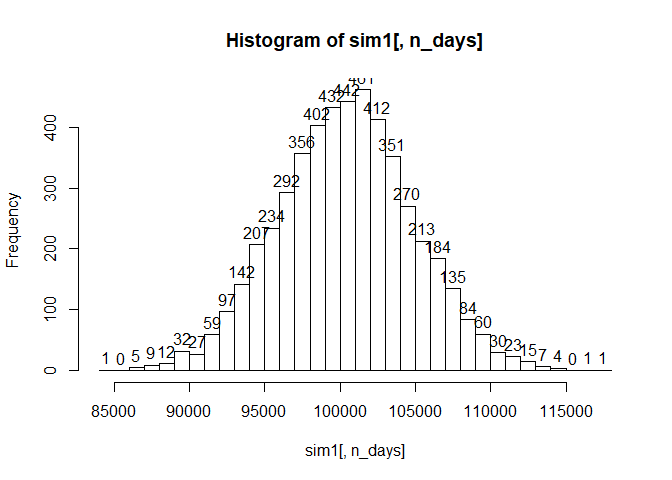
\includegraphics{finalproj_files/figure-latex/unnamed-chunk-9-1.pdf}

\begin{Shaded}
\begin{Highlighting}[]
\NormalTok{VAR =}\StringTok{ }\KeywordTok{quantile}\NormalTok{(sim1[,n_days], }\FloatTok{.05}\NormalTok{)}
\NormalTok{VAR}
\end{Highlighting}
\end{Shaded}

\begin{verbatim}
##       5% 
## 93091.06
\end{verbatim}

Second Portfolio

\begin{Shaded}
\begin{Highlighting}[]
\NormalTok{initial_wealth =}\StringTok{ }\DecValTok{100000}
\NormalTok{sim2 =}\StringTok{ }\KeywordTok{foreach}\NormalTok{(}\DataTypeTok{i =} \DecValTok{1}\OperatorTok{:}\DecValTok{5000}\NormalTok{, }\DataTypeTok{.combine =} \StringTok{"rbind"}\NormalTok{)}\OperatorTok\NormalTok{\{}
\NormalTok{  total_wealth_b =}\StringTok{ }\NormalTok{initial_wealth}
  
\NormalTok{  my_weights_b <-}\StringTok{ }\KeywordTok{c}\NormalTok{(}\FloatTok{0.25}\NormalTok{, }\FloatTok{0.25}\NormalTok{, }\FloatTok{0.25}\NormalTok{, }\FloatTok{0.25}\NormalTok{)}
  
\NormalTok{  holdings_b <-}\StringTok{ }\NormalTok{my_weights_b}\OperatorTok{*}\NormalTok{total_wealth_b}
  
\NormalTok{  n_days =}\StringTok{ }\DecValTok{20}
  
\NormalTok{  wealthtracker_b =}\StringTok{ }\KeywordTok{rep}\NormalTok{(}\DecValTok{0}\NormalTok{, n_days)}
  
  \ControlFlowTok{for}\NormalTok{(today }\ControlFlowTok{in} \DecValTok{1}\OperatorTok{:}\NormalTok{n_days)\{}
\NormalTok{    return.today_b <-}\StringTok{ }\KeywordTok{resample}\NormalTok{(all_returns_b, }\DecValTok{1}\NormalTok{, }\DataTypeTok{orig.ids =} \OtherTok{FALSE}\NormalTok{)}
  
\NormalTok{    holdings_b <-}\StringTok{ }\NormalTok{holdings_b}\OperatorTok{*}\NormalTok{(}\DecValTok{1}\OperatorTok{+}\NormalTok{return.today_b)}
  
\NormalTok{    total_wealth_b <-}\StringTok{ }\KeywordTok{sum}\NormalTok{(holdings_b)}
  
\NormalTok{    wealthtracker_b[today] =}\StringTok{ }\NormalTok{total_wealth_b}
\NormalTok{  \}}
\NormalTok{  wealthtracker_b}

  
\NormalTok{\}}
\KeywordTok{head}\NormalTok{(sim2)}
\end{Highlighting}
\end{Shaded}

\begin{verbatim}
##               [,1]      [,2]     [,3]      [,4]      [,5]      [,6]
## result.1 100401.31 100445.02 100924.8 101131.75 101425.45 101579.75
## result.2 100643.01 101162.64 102082.0 100915.41 101881.84 101213.82
## result.3 100625.01 101113.20 102271.8 101651.05 102346.48 101581.00
## result.4 101910.46 100142.62 100017.0  99584.09 100114.65 100461.78
## result.5 100237.85 101362.94 102536.5 101822.51 102027.67 103196.52
## result.6  99748.39  99091.21  99927.3  99888.92  99330.26  99238.78
##               [,7]      [,8]      [,9]     [,10]     [,11]     [,12]
## result.1  99687.99  99239.12  99440.91  94951.75  95684.82  95498.22
## result.2 100982.24  99510.99  99951.17  99097.45 100466.26 100543.49
## result.3 103216.83 103699.44 104824.97 103036.30 102862.11 103367.80
## result.4 100423.46  99779.07 100426.54  98681.73  98843.99  98786.97
## result.5 103340.80 104048.19 103680.11 104080.97 104842.12 104946.09
## result.6  97974.54  97577.76  96339.87  96565.82  96420.10  95934.32
##              [,13]     [,14]     [,15]     [,16]     [,17]     [,18]
## result.1  96233.18  96757.95  97064.97  97667.21  97612.28  97656.52
## result.2  99940.25 100931.23 100976.66 100085.62  99683.01  99698.92
## result.3 103941.22 103939.81 104180.18 103102.17 103931.54 105247.93
## result.4  98689.94  96585.16  95696.20  94708.07  95154.47  94998.99
## result.5 104731.50 105236.81 104213.43 104867.79 105946.46 106624.22
## result.6  96690.17  96555.68  96702.64  96340.25  95619.09  96013.66
##              [,19]     [,20]
## result.1  98033.27  98817.79
## result.2  97056.02  97110.64
## result.3 103877.55 103809.67
## result.4  92593.40  92871.78
## result.5 107156.68 106798.18
## result.6  95963.21  95897.04
\end{verbatim}

\begin{Shaded}
\begin{Highlighting}[]
\KeywordTok{hist}\NormalTok{(sim2[,n_days], }\DecValTok{25}\NormalTok{)}
\end{Highlighting}
\end{Shaded}

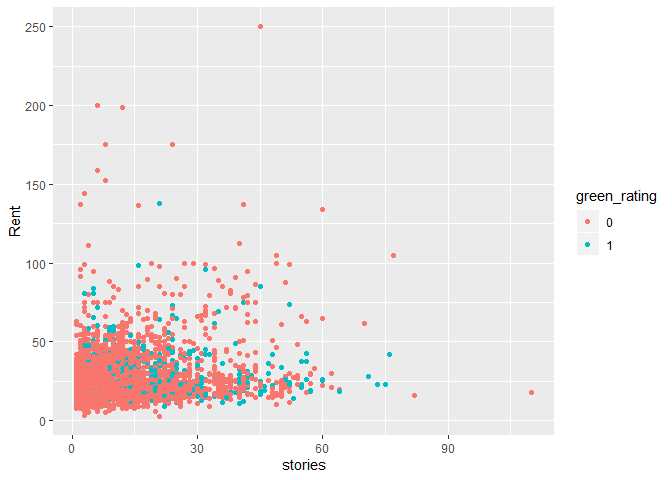
\includegraphics{finalproj_files/figure-latex/unnamed-chunk-10-1.pdf}

\begin{Shaded}
\begin{Highlighting}[]
\NormalTok{VAR =}\StringTok{ }\KeywordTok{quantile}\NormalTok{(sim2[,n_days], }\FloatTok{.05}\NormalTok{)}
\NormalTok{VAR}
\end{Highlighting}
\end{Shaded}

\begin{verbatim}
##       5% 
## 93291.91
\end{verbatim}

Portfolio C

\begin{Shaded}
\begin{Highlighting}[]
\NormalTok{initial_wealth =}\StringTok{ }\DecValTok{100000}
\NormalTok{sim3 =}\StringTok{ }\KeywordTok{foreach}\NormalTok{(}\DataTypeTok{i =} \DecValTok{1}\OperatorTok{:}\DecValTok{5000}\NormalTok{, }\DataTypeTok{.combine =} \StringTok{"rbind"}\NormalTok{)}\OperatorTok\NormalTok{\{}
\NormalTok{  total_wealth_c =}\StringTok{ }\NormalTok{initial_wealth}
  
\NormalTok{  my_weights_c <-}\StringTok{ }\KeywordTok{c}\NormalTok{(}\FloatTok{0.14}\NormalTok{, }\FloatTok{0.14}\NormalTok{, }\FloatTok{0.15}\NormalTok{, }\FloatTok{0.14}\NormalTok{, }\FloatTok{0.14}\NormalTok{, }\FloatTok{0.14}\NormalTok{, }\FloatTok{0.15}\NormalTok{)}
  
\NormalTok{  holdings_c <-}\StringTok{ }\NormalTok{my_weights_c}\OperatorTok{*}\NormalTok{total_wealth_c}
  
\NormalTok{  n_days =}\StringTok{ }\DecValTok{20}
  
\NormalTok{  wealthtracker_c =}\StringTok{ }\KeywordTok{rep}\NormalTok{(}\DecValTok{0}\NormalTok{, n_days)}
  
  \ControlFlowTok{for}\NormalTok{(today }\ControlFlowTok{in} \DecValTok{1}\OperatorTok{:}\NormalTok{n_days)\{}
\NormalTok{    return.today_c <-}\StringTok{ }\KeywordTok{resample}\NormalTok{(all_returns_c, }\DecValTok{1}\NormalTok{, }\DataTypeTok{orig.ids =} \OtherTok{FALSE}\NormalTok{)}
  
\NormalTok{    holdings_c <-}\StringTok{ }\NormalTok{holdings_c}\OperatorTok{*}\NormalTok{(}\DecValTok{1}\OperatorTok{+}\NormalTok{return.today_c)}
  
\NormalTok{    total_wealth_c <-}\StringTok{ }\KeywordTok{sum}\NormalTok{(holdings_c)}
  
\NormalTok{    wealthtracker_c[today] =}\StringTok{ }\NormalTok{total_wealth_c}
\NormalTok{  \}}
\NormalTok{  wealthtracker_c}

  
\NormalTok{\}}
\KeywordTok{head}\NormalTok{(sim3)}
\end{Highlighting}
\end{Shaded}

\begin{verbatim}
##               [,1]     [,2]      [,3]      [,4]      [,5]      [,6]
## result.1  99617.01 100147.7  99494.07  99796.72 100021.52  99955.32
## result.2  98591.44  97550.6  96626.22  97254.93  97082.22  96691.90
## result.3 100145.56 100132.5  97396.47  97163.97  95906.18  96140.94
## result.4 100636.24 101583.1 101799.15 101047.61 101410.39 104498.02
## result.5 100265.29 100107.5 101344.61 101521.10 102789.98 104384.57
## result.6 101274.17 101697.6 102661.99 102515.70 101793.65 100369.16
##               [,7]      [,8]      [,9]     [,10]     [,11]     [,12]
## result.1 100371.73 101701.02 101727.99 100026.38 100981.67 101441.06
## result.2  97265.25  90717.37  90574.09  89653.96  89074.00  88933.96
## result.3  96514.18  96485.20  96535.61  97150.72  96495.25  95511.61
## result.4 104305.12 104372.45 104431.70 104243.17 103417.97 103413.39
## result.5 106606.93 105840.50 105521.63 102766.10 103229.47 104226.13
## result.6 101490.78 101315.66 100522.35 100295.82  99486.12  97576.96
##              [,13]     [,14]     [,15]     [,16]     [,17]     [,18]
## result.1 100662.48 100572.20 100037.68 100600.59 101100.91 102138.67
## result.2  87997.67  87543.49  87937.34  89963.33  89655.30  90644.85
## result.3  96409.93  95292.50  94893.22  96011.52  95785.37  95957.99
## result.4 103968.18 104647.20 105750.25 105059.75 106737.86 106747.48
## result.5 104260.43 104271.73 104328.95 101760.91  99608.07 100612.21
## result.6  96993.69  94974.79  95345.08  95362.55  94031.77  95896.80
##              [,19]     [,20]
## result.1 103696.85 103460.24
## result.2  90574.02  89999.99
## result.3  94483.27  93918.35
## result.4 106582.43 107638.79
## result.5 100856.23 100777.91
## result.6  96574.88  96531.93
\end{verbatim}

\begin{Shaded}
\begin{Highlighting}[]
\KeywordTok{hist}\NormalTok{(sim3[,n_days], }\DecValTok{25}\NormalTok{)}
\end{Highlighting}
\end{Shaded}

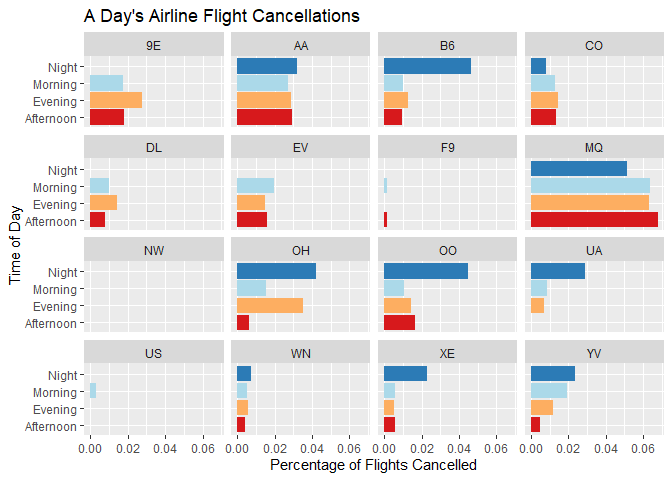
\includegraphics{finalproj_files/figure-latex/unnamed-chunk-11-1.pdf}

\begin{Shaded}
\begin{Highlighting}[]
\NormalTok{VAR =}\StringTok{ }\KeywordTok{quantile}\NormalTok{(sim3[,n_days], }\FloatTok{.05}\NormalTok{)}
\NormalTok{VAR}
\end{Highlighting}
\end{Shaded}

\begin{verbatim}
##       5% 
## 91864.87
\end{verbatim}

I selected the portfolios with the intention of giving each one a
different aim, despite all of the ETF's being chosen from either the
China ETF category, the Japan ETF category, Euro ETF category, or the
Emerging Markets category. The first portfolio was chosen by being
comprised of ETF's which have the highest previous day's closing cost.
It contained 5 ETF's (EDEN, GXC, CXSE, QEMM, and IEMG), with closing
costs ranging from \$47.99 to \$87.82. The second portfolio contained 4
ETF's (FSZ, JPMV, FCA, and TUR), and those ETF's were chosen with the
aim of minimizing the percent change from the previous day (in order to
minimize short-term volatility). The third portfolio contained 7 ETF's
(EWJ, EWL, EWN, ASHR, KFYP, GREK, and ERUS), and were chosen with the
intention of maximizing YTD, in order to maximize long-term growth.


\end{document}
